\chapter{Slope Fields}

While separable differential equations are solvable, most differential 
equations are not separable. In fact, it is impossible to obtain an 
explicit formula as a solution to most differential equations. How do computers 
solve these, then? They start with a given quantity (usually initial 
conditions) and perform many small calculations to estimate the behavior of 
the solution. We can do this graphically with slope fields (also called 
direction fields), which allow us to visualize the family of solutions to the 
differential equation. \index{slope field}

\section{Drawing Slope Fields}
When a differential equation is in the form
$$y' = f(x,y)$$
we can use the coordinates $(x,y)$ to determine the slope of a solution to the 
differential equation at that coordinate. Take $y' = x + y$ as an example. 
According to this differential equation, a solution that passes through the 
point $(1, 1)$ would have a slope of $2$. We can represent this with a small 
tick of slope $2$ at the $(1, 1)$ (see figure \ref{slopefield1}). 

\begin{figure}[htbp]
\centering
    \begin{tikzpicture}
	\begin{axis}[xmin = -3, xmax = 3, ymin = -3, ymax = 3, 
	ytick = {-3, -2, -1, 1, 2, 3}, xtick = {-3, -2, -1, 1, 2, 3}, xlabel = $x$, 
	ylabel = $y$, axis lines = center]
	\draw[blue, thin](0.9, 0.8) -- (1.1, 1.2);
        \end{axis}
    \end{tikzpicture}
    \caption{A solution to $y' = x + y$ that passes through $(1,1)$ will have 
    a slope of $2$ at that point}
    \label{slopefield1}
\end{figure}

Continuing, we want to choose coordinates that are easy to determine the slope. 
Notice that $y' = 0$ when $-x = y$, so let's go ahead and fill those ticks in 
(see figure \ref{slopefield2}):

\begin{figure}[htbp]
\centering
    \begin{tikzpicture}
	\begin{axis}[xmin = -3.1, xmax = 3.1, ymin = -3.1, ymax = 3.1, 
	ytick = {-3, -2, -1, 1, 2, 3}, xtick = {-3, -2, -1, 1, 2, 3}, xlabel = $x$, 
	ylabel = $y$, axis lines = center]
	\draw[blue, thin](0.9, 0.8) -- (1.1, 1.2);
        \draw[blue, thin] (-0.9, 1) -- (-1.1, 1);
        \draw[blue, thin] (-1.9, 2) -- (-2.1, 2);
        \draw[blue, thin] (-2.9, 3) -- (-3.1, 3);
        \draw[blue, thin] (-0.1, 0) -- (0.1, 0);
        \draw[blue, thin] (0.9, -1) -- (1.1, -1);
        \draw[blue, thin] (1.9, -2) -- (2.1, -2);
        \draw[blue, thin] (2.9, -3) -- (3.1, -3);
        \end{axis}
    \end{tikzpicture}
    \caption{Solutions to $y'=x+y$ that lie on the line $y = -x$ will have a 
    slope of $0$.}
    \label{slopefield2}
\end{figure}

We can repeat this process for all the coordinates shown, resulting in a slope 
field (see figure \ref{slopefield3}).

\begin{figure}[htbp]
\centering
    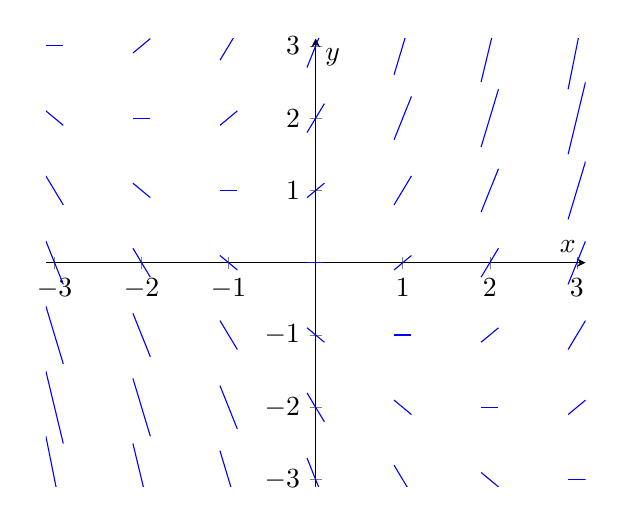
\begin{tikzpicture}
	\begin{axis}[xmin = -3.1, xmax = 3.1, ymin = -3.1, ymax = 3.1, 
	ytick = {-3, -2, -1, 1, 2, 3}, xtick = {-3, -2, -1, 1, 2, 3}, xlabel = $x$, 
	ylabel = $y$, axis lines = center]
	\draw[blue, thin](0.9, 0.8) -- (1.1, 1.2);
        \draw[blue, thin] (-0.9, 1) -- (-1.1, 1);
        \draw[blue, thin] (-1.9, 2) -- (-2.1, 2);
        \draw[blue, thin] (-2.9, 3) -- (-3.1, 3);
        \draw[blue, thin] (-0.1, 0) -- (0.1, 0);
        \draw[blue, thin] (0.9, -1) -- (1.1, -1);
        \draw[blue, thin] (1.9, -2) -- (2.1, -2);
        \draw[blue, thin] (2.9, -3) -- (3.1, -3);
        \draw[blue, thin] (-3.1, -2.4) -- (-2.9, -3.6);
        \draw[blue, thin] (-3.1, -1.5) -- (-2.9, -2.5);
        \draw[blue, thin] (-3.1, -0.6) -- (-2.9, -1.4);
        \draw[blue, thin] (-3.1, 0.3) -- (-2.9, -0.3);
        \draw[blue, thin] (-3.1, 1.2) -- (-2.9, 0.8);
        \draw[blue, thin] (-3.1, 2.1) -- (-2.9, 1.9);
        \draw[blue, thin] (-2.1, -2.5) -- (-1.9, -3.5);
        \draw[blue, thin] (-2.1, -1.6) -- (-1.9, -2.4);
        \draw[blue, thin] (-2.1, -0.7) -- (-1.9, -1.3);
        \draw[blue, thin] (-2.1, 0.2) -- (-1.9, -0.2);
        \draw[blue, thin] (-2.1, 1.1) -- (-1.9, 0.9);
        \draw[blue, thin] (-2.1, 2.9) -- (-1.9, 3.1);
        \draw[blue, thin] (-1.1, -2.6) -- (-0.9, -3.4);
        \draw[blue, thin] (-1.1, -1.7) -- (-0.9, -2.3);
        \draw[blue, thin] (-1.1, -0.8) -- (-0.9, -1.2);
        \draw[blue, thin] (-1.1, 0.1) -- (-0.9, -0.1);
        \draw[blue, thin] (-1.1, 1.9) -- (-0.9, 2.1);
        \draw[blue, thin] (-1.1, 2.8) -- (-0.9, 3.2);
        \draw[blue, thin] (-0.1, -2.7) -- (0.1, -3.3);
        \draw[blue, thin] (-0.1, -1.8) -- (0.1, -2.2);
        \draw[blue, thin] (-0.1, -0.9) -- (0.1, -1.1);
        \draw[blue, thin] (-0.1, 0.9) -- (0.1, 1.1);
        \draw[blue, thin] (-0.1, 1.8) -- (0.1, 2.2);
        \draw[blue, thin] (-0.1, 2.7) -- (0.1, 3.3);
        \draw[blue, thin] (0.9, -2.8) -- (1.1, -3.2);
        \draw[blue, thin] (0.9, -1.9) -- (1.1, -2.1);
        \draw[blue, thin] (0.9, -0.1) -- (1.1, 0.1);
        \draw[blue, thin] (0.9, 1.7) -- (1.1, 2.3);
        \draw[blue, thin] (0.9, 2.6) -- (1.1, 3.4);
        \draw[blue, thin] (1.9, -2.9) -- (2.1, -3.1);
        \draw[blue, thin] (1.9, -1.1) -- (2.1, -0.9);
        \draw[blue, thin] (1.9, -0.2) -- (2.1, 0.2);
        \draw[blue, thin] (1.9, 0.7) -- (2.1, 1.3);
        \draw[blue, thin] (1.9, 1.6) -- (2.1, 2.4);
        \draw[blue, thin] (1.9, 2.5) -- (2.1, 3.5);
        \draw[blue, thin] (2.9, -2.1) -- (3.1, -1.9);
        \draw[blue, thin] (2.9, -1.2) -- (3.1, -0.8);
        \draw[blue, thin] (2.9, -0.3) -- (3.1, 0.3);
        \draw[blue, thin] (2.9, 0.6) -- (3.1, 1.4);
        \draw[blue, thin] (2.9, 1.5) -- (3.1, 2.5);
        \draw[blue, thin] (2.9, 2.4) -- (3.1, 3.6);
        \end{axis}
    \end{tikzpicture}
    \caption{Slope field of $y'=x+y$}
    \label{slopefield3}
\end{figure}

\section{Sketching solutions on slope fields}

If you are given an initial condition or a known point in the solution to the 
differential equation, you can begin sketching a curve on the slope field. 
Start at the given point and draw parallel to the nearby slopes. For example, 
suppose we know that particular solution to $y' = x + y$ passes through the 
point $(1, 0)$. Begin by extending the dash at $(1, 0)$ (see figure 
\ref{slopefield4}), changing the slope of your sketched solution to be 
approximately parallel to the nearby slopes (see figure \ref{slopefield5}). 

\begin{figure}[htbp]
\centering
    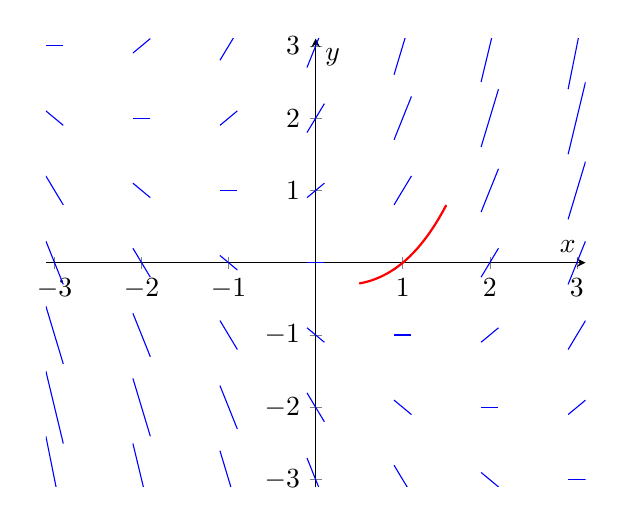
\begin{tikzpicture}
	\begin{axis}[xmin = -3.1, xmax = 3.1, ymin = -3.1, ymax = 3.1, 
	ytick = {-3, -2, -1, 1, 2, 3}, xtick = {-3, -2, -1, 1, 2, 3}, xlabel = $x$, 
	ylabel = $y$, axis lines = center]
	\draw[blue, thin](0.9, 0.8) -- (1.1, 1.2);
        \draw[blue, thin] (-0.9, 1) -- (-1.1, 1);
        \draw[blue, thin] (-1.9, 2) -- (-2.1, 2);
        \draw[blue, thin] (-2.9, 3) -- (-3.1, 3);
        \draw[blue, thin] (-0.1, 0) -- (0.1, 0);
        \draw[blue, thin] (0.9, -1) -- (1.1, -1);
        \draw[blue, thin] (1.9, -2) -- (2.1, -2);
        \draw[blue, thin] (2.9, -3) -- (3.1, -3);
        \draw[blue, thin] (-3.1, -2.4) -- (-2.9, -3.6);
        \draw[blue, thin] (-3.1, -1.5) -- (-2.9, -2.5);
        \draw[blue, thin] (-3.1, -0.6) -- (-2.9, -1.4);
        \draw[blue, thin] (-3.1, 0.3) -- (-2.9, -0.3);
        \draw[blue, thin] (-3.1, 1.2) -- (-2.9, 0.8);
        \draw[blue, thin] (-3.1, 2.1) -- (-2.9, 1.9);
        \draw[blue, thin] (-2.1, -2.5) -- (-1.9, -3.5);
        \draw[blue, thin] (-2.1, -1.6) -- (-1.9, -2.4);
        \draw[blue, thin] (-2.1, -0.7) -- (-1.9, -1.3);
        \draw[blue, thin] (-2.1, 0.2) -- (-1.9, -0.2);
        \draw[blue, thin] (-2.1, 1.1) -- (-1.9, 0.9);
        \draw[blue, thin] (-2.1, 2.9) -- (-1.9, 3.1);
        \draw[blue, thin] (-1.1, -2.6) -- (-0.9, -3.4);
        \draw[blue, thin] (-1.1, -1.7) -- (-0.9, -2.3);
        \draw[blue, thin] (-1.1, -0.8) -- (-0.9, -1.2);
        \draw[blue, thin] (-1.1, 0.1) -- (-0.9, -0.1);
        \draw[blue, thin] (-1.1, 1.9) -- (-0.9, 2.1);
        \draw[blue, thin] (-1.1, 2.8) -- (-0.9, 3.2);
        \draw[blue, thin] (-0.1, -2.7) -- (0.1, -3.3);
        \draw[blue, thin] (-0.1, -1.8) -- (0.1, -2.2);
        \draw[blue, thin] (-0.1, -0.9) -- (0.1, -1.1);
        \draw[blue, thin] (-0.1, 0.9) -- (0.1, 1.1);
        \draw[blue, thin] (-0.1, 1.8) -- (0.1, 2.2);
        \draw[blue, thin] (-0.1, 2.7) -- (0.1, 3.3);
        \draw[blue, thin] (0.9, -2.8) -- (1.1, -3.2);
        \draw[blue, thin] (0.9, -1.9) -- (1.1, -2.1);
        \draw[blue, thin] (0.9, -0.1) -- (1.1, 0.1);
        \draw[blue, thin] (0.9, 1.7) -- (1.1, 2.3);
        \draw[blue, thin] (0.9, 2.6) -- (1.1, 3.4);
        \draw[blue, thin] (1.9, -2.9) -- (2.1, -3.1);
        \draw[blue, thin] (1.9, -1.1) -- (2.1, -0.9);
        \draw[blue, thin] (1.9, -0.2) -- (2.1, 0.2);
        \draw[blue, thin] (1.9, 0.7) -- (2.1, 1.3);
        \draw[blue, thin] (1.9, 1.6) -- (2.1, 2.4);
        \draw[blue, thin] (1.9, 2.5) -- (2.1, 3.5);
        \draw[blue, thin] (2.9, -2.1) -- (3.1, -1.9);
        \draw[blue, thin] (2.9, -1.2) -- (3.1, -0.8);
        \draw[blue, thin] (2.9, -0.3) -- (3.1, 0.3);
        \draw[blue, thin] (2.9, 0.6) -- (3.1, 1.4);
        \draw[blue, thin] (2.9, 1.5) -- (3.1, 2.5);
        \draw[blue, thin] (2.9, 2.4) -- (3.1, 3.6);
        \addplot[red, thick, domain = 0.5:1.5]{-1*x + 2*e^(x - 1) - 1};
        \end{axis}
    \end{tikzpicture}
    \caption{To begin sketching a solution to the differential equation, start 
    at the point given as part of the solution}
    \label{slopefield4}
\end{figure}

\begin{figure}[htbp]
\centering
    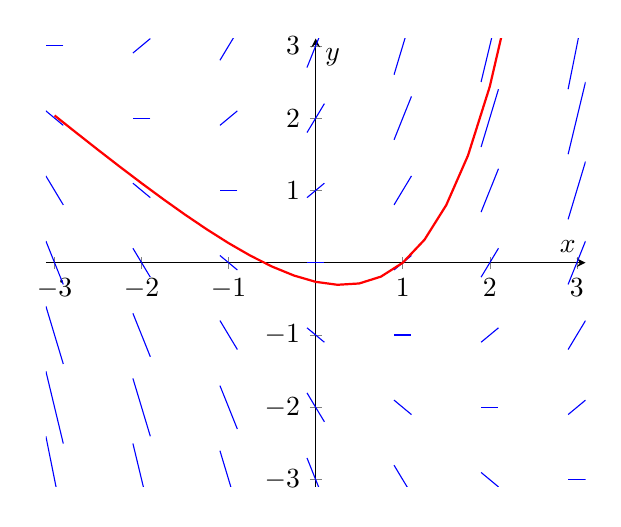
\begin{tikzpicture}
	\begin{axis}[xmin = -3.1, xmax = 3.1, ymin = -3.1, ymax = 3.1, 
	ytick = {-3, -2, -1, 1, 2, 3}, xtick = {-3, -2, -1, 1, 2, 3}, xlabel = $x$, 
	ylabel = $y$, axis lines = center]
	\draw[blue, thin](0.9, 0.8) -- (1.1, 1.2);
        \draw[blue, thin] (-0.9, 1) -- (-1.1, 1);
        \draw[blue, thin] (-1.9, 2) -- (-2.1, 2);
        \draw[blue, thin] (-2.9, 3) -- (-3.1, 3);
        \draw[blue, thin] (-0.1, 0) -- (0.1, 0);
        \draw[blue, thin] (0.9, -1) -- (1.1, -1);
        \draw[blue, thin] (1.9, -2) -- (2.1, -2);
        \draw[blue, thin] (2.9, -3) -- (3.1, -3);
        \draw[blue, thin] (-3.1, -2.4) -- (-2.9, -3.6);
        \draw[blue, thin] (-3.1, -1.5) -- (-2.9, -2.5);
        \draw[blue, thin] (-3.1, -0.6) -- (-2.9, -1.4);
        \draw[blue, thin] (-3.1, 0.3) -- (-2.9, -0.3);
        \draw[blue, thin] (-3.1, 1.2) -- (-2.9, 0.8);
        \draw[blue, thin] (-3.1, 2.1) -- (-2.9, 1.9);
        \draw[blue, thin] (-2.1, -2.5) -- (-1.9, -3.5);
        \draw[blue, thin] (-2.1, -1.6) -- (-1.9, -2.4);
        \draw[blue, thin] (-2.1, -0.7) -- (-1.9, -1.3);
        \draw[blue, thin] (-2.1, 0.2) -- (-1.9, -0.2);
        \draw[blue, thin] (-2.1, 1.1) -- (-1.9, 0.9);
        \draw[blue, thin] (-2.1, 2.9) -- (-1.9, 3.1);
        \draw[blue, thin] (-1.1, -2.6) -- (-0.9, -3.4);
        \draw[blue, thin] (-1.1, -1.7) -- (-0.9, -2.3);
        \draw[blue, thin] (-1.1, -0.8) -- (-0.9, -1.2);
        \draw[blue, thin] (-1.1, 0.1) -- (-0.9, -0.1);
        \draw[blue, thin] (-1.1, 1.9) -- (-0.9, 2.1);
        \draw[blue, thin] (-1.1, 2.8) -- (-0.9, 3.2);
        \draw[blue, thin] (-0.1, -2.7) -- (0.1, -3.3);
        \draw[blue, thin] (-0.1, -1.8) -- (0.1, -2.2);
        \draw[blue, thin] (-0.1, -0.9) -- (0.1, -1.1);
        \draw[blue, thin] (-0.1, 0.9) -- (0.1, 1.1);
        \draw[blue, thin] (-0.1, 1.8) -- (0.1, 2.2);
        \draw[blue, thin] (-0.1, 2.7) -- (0.1, 3.3);
        \draw[blue, thin] (0.9, -2.8) -- (1.1, -3.2);
        \draw[blue, thin] (0.9, -1.9) -- (1.1, -2.1);
        \draw[blue, thin] (0.9, -0.1) -- (1.1, 0.1);
        \draw[blue, thin] (0.9, 1.7) -- (1.1, 2.3);
        \draw[blue, thin] (0.9, 2.6) -- (1.1, 3.4);
        \draw[blue, thin] (1.9, -2.9) -- (2.1, -3.1);
        \draw[blue, thin] (1.9, -1.1) -- (2.1, -0.9);
        \draw[blue, thin] (1.9, -0.2) -- (2.1, 0.2);
        \draw[blue, thin] (1.9, 0.7) -- (2.1, 1.3);
        \draw[blue, thin] (1.9, 1.6) -- (2.1, 2.4);
        \draw[blue, thin] (1.9, 2.5) -- (2.1, 3.5);
        \draw[blue, thin] (2.9, -2.1) -- (3.1, -1.9);
        \draw[blue, thin] (2.9, -1.2) -- (3.1, -0.8);
        \draw[blue, thin] (2.9, -0.3) -- (3.1, 0.3);
        \draw[blue, thin] (2.9, 0.6) -- (3.1, 1.4);
        \draw[blue, thin] (2.9, 1.5) -- (3.1, 2.5);
        \draw[blue, thin] (2.9, 2.4) -- (3.1, 3.6);
        \addplot[red, thick, domain = -3:3]{-1*x + 2*e^(x - 1) - 1};
        \end{axis}
    \end{tikzpicture}
    \caption{To sketch a solution to the differential equation, draw a function 
    parallel to the nearby slopes that passes through the given point in the 
    particular solution}
    \label{slopefield5}
\end{figure}

While this method doesn't yield an exact, formulaic solution to the 
differential equation, it does allow us to visualize solutions and generally 
describe the behavior of any solutions. Sketching solutions in this way is 
logically similar to Euler's method for finding numerical approximations of 
solutions to differential equations, which we will discuss more in the next 
chapter. 

\section{Example: Application of Differential Equations to Electronics}
Think back to the chapter on DC circuits. You learned that Ohm's Law relates 
voltage (electromotive force), current, and resistance for simple DC circuits:
$$V = IR$$

Simple resistors have a constant resistance, so once the voltage source 
(battery) is connected, the current is constant. There are other electronic 
components, such as inductors and capacitors, that behave differently. When 
current changes in an inductor, a voltage drop is induced across the inductor. 
This is described by the differential equation:
$$V = -L\frac{dI}{dt}$$
Where $L$ is inductance, measured in henries (H), of the inductor. Consider, 
then, a circuit consisting of a constant-voltage battery, a fixed resistor, 
and an inductor (shown in figure \ref{circuit}). Since Kirchoff's Law states 
that the sum of the voltage drops across each component must equal the voltage 
supplied by the battery, we can write a differential equation to describe the 
circuit:
$$V = L\frac{dI}{dt} + RI$$

Where the current, I, is a function of time, t. 

\begin{figure}[htbp]
\centering
    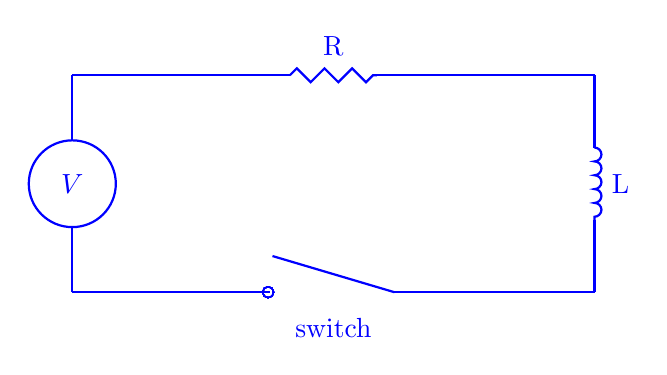
\begin{tikzpicture}
	\begin{axis}[xmin = -3.1, xmax = 3.1, ymin = -3.1, ymax = 3.1, axis lines = 
	none, clip = false]
	\draw[blue, thick](-3, 1.5) -- (-0.5, 1.5);
        \draw[blue, thick] (0.5, 1.5) -- (3, 1.5);
        \draw[decorate, decoration = zigzag, color=blue, thick] 
        	(-0.5, 1.5) -- (0.5, 1.5);
        \draw[blue, thick](3,1.5) -- (3, 0.5);
        \draw[decorate, decoration = bumps, color=blue, thick] 
        	(3, 0.5) -- (3, -0.5);
        \draw[blue, thick] (3, -0.5) -- (3, -1.5);
        \draw[blue, thick] (3, -1.5) -- (0.7, -1.5);
        \draw[blue, thick] (0.7, -1.5) -- (-0.7, -1);
        \draw[blue, thick] (-0.73, -1.5) -- (-3, -1.5);
        \addplot[blue, mark=o](-0.75, -1.5);
        \draw[blue, thick] (-3, -1.5) -- (-3, -0.6);
        \draw[blue, thick] (-3, 0.6) -- (-3, 1.5);
        \draw[blue, thick] (-3, 0) ellipse (0.5 and 0.6);
        \node[blue] at (-3, 0) {$V$};
        \node[blue] at (0, -2) {switch};
        \node[blue] at (3.3, 0) {L};
        \node[blue] at (0, 1.9) {R};
        \end{axis}
    \end{tikzpicture}
    \caption{A simple circuit with a battery, resistor, inductor, and switch}
    \label{circuit}
\end{figure}

\textbf{Example}: If the resistor is $12 \Omega$, the inductance is $4H$, and 
the battery supplies a constant voltage of $60V$:
\begin{enumerate}
\item Draw a slope field for the differential equation describing the current 
in the circuit.
\item Describe the expected behavior of the current over a long period of time.
\item Identify any equilibrium solutions.
\item If the initial current at $t = 0$ is $I(0) = 0$, sketch the particular 
solution to the differential equation on the slope field. 
\end{enumerate}

\textbf{Solution}: Substituting the given values into the differential 
equation and rearranging to isolate $\frac{dI}{dt}$, we get $\frac{dI}{dt} = 
15 - 3I$. Notice that the current is not dependent on time. When the slope is 
only dependent on the value of the function (as in this case), we call this an 
\textbf{autonomous differential equation}. \index{autonomous differential 
equation} This means that the slope will be the same of all values of $t$ for 
a given $I$. The slope field is shown in figure \ref{circuitslope}. 

\begin{figure}[htbp]
\centering
    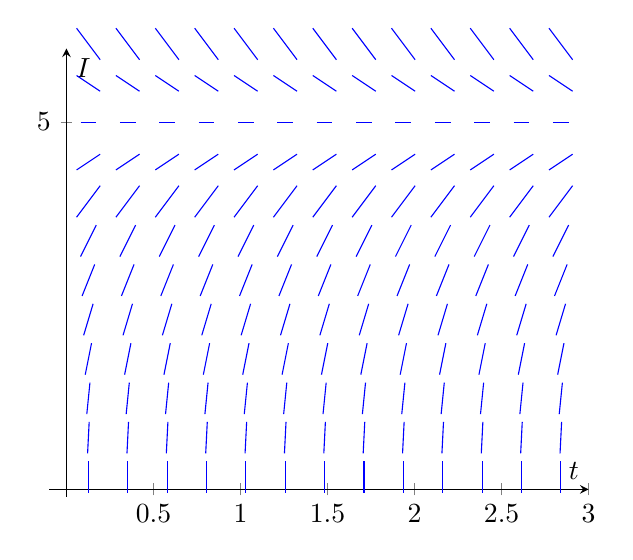
\begin{tikzpicture}
    \begin{axis}[xmin = -0.1, xmax = 3, ymin = -0.1, ymax = 6, axis lines = 
    center, xlabel = $t$, ylabel = $I$, ytick = 5]
    \end{axis}
	
        \foreach \x in {1, 2,..., 13}{
        \draw[blue, thin](\x/2 - 0.15, 5.75 + 0.2) -- (\x/2 + 0.15, 5.75 - 0.2);
        \draw[blue, thin](\x/2 - 0.15, 5.25 + 0.1) -- (\x/2 + 0.15, 5.25 - 0.1);
        \draw[blue, thin](\x/2 - 0.1, 4.75) -- (\x/2 + 0.1, 4.75);
        \draw[blue, thin](\x/2 - 0.15, 4.25 - 0.1) -- (\x/2 + 0.15, 4.25 + 0.1);
        \draw[blue, thin](\x/2 - 0.15, 3.75 - 0.2) -- (\x/2 + 0.15, 3.75 + 0.2);
        \draw[blue, thin](\x/2 - 0.1, 3.25 - 0.2) -- (\x/2 + 0.1, 3.25 + 0.2);
        \draw[blue, thin](\x/2 - 0.08, 2.75 - 0.2) -- (\x/2 + 0.08, 2.75 + 0.2);
        \draw[blue, thin](\x/2 - 0.06, 2.25 - 0.2) -- (\x/2 + 0.06, 2.25 + 0.2);
        \draw[blue, thin](\x/2 - 0.04, 1.75 - 0.2) -- (\x/2 + 0.04, 1.75 + 0.2);
        \draw[blue, thin](\x/2 - 0.02, 1.25 - 0.2) -- (\x/2 + 0.02, 1.25 + 0.2);
        \draw[blue, thin](\x/2 - 0.01, 0.75 - 0.2) -- (\x/2 + 0.01, 0.75 + 0.2);
        \draw[blue, thin](\x/2, 0.25 - 0.2) -- (\x/2, 0.25 + 0.2);
        }
        
    \end{tikzpicture}
    \caption{Slope field for the differential equation $\frac{dI}{dt} = 15 - 3I$}
    \label{circuitslope}
\end{figure}

Examining the slope field, we see that the solutions tend towards $I(t) = 5$, 
which suggests that over an extended period of time, the current will approach 
5 amperes. Similarly, if the initial current were 5 amperes, then the current 
would be constant at 5 amperes. Therefore, $I(t) = 5$ is an equilibrium 
solution. A sketch of the solution with $I(0) = 0$ is shown in figure 
\ref{circuitsolution}. 

\begin{figure}[htbp]
\centering
    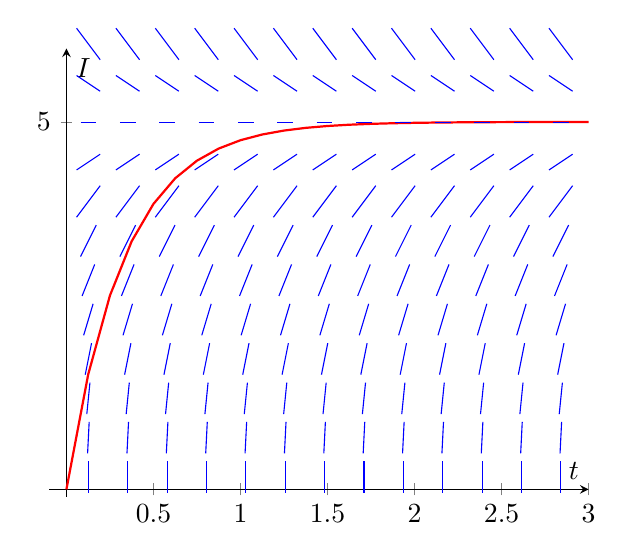
\begin{tikzpicture}
    \begin{axis}[xmin = -0.1, xmax = 3, ymin = -0.1, ymax = 6, axis lines = 
    center, xlabel = $t$, ylabel = $I$, ytick = 5]
    \addplot[red, thick,, domain = 0:3]{5 - 5*e^(-3*x)};
    \end{axis}
	
        \foreach \x in {1, 2,..., 13}{
        \draw[blue, thin](\x/2 - 0.15, 5.75 + 0.2) -- (\x/2 + 0.15, 5.75 - 0.2);
        \draw[blue, thin](\x/2 - 0.15, 5.25 + 0.1) -- (\x/2 + 0.15, 5.25 - 0.1);
        \draw[blue, thin](\x/2 - 0.1, 4.75) -- (\x/2 + 0.1, 4.75);
        \draw[blue, thin](\x/2 - 0.15, 4.25 - 0.1) -- (\x/2 + 0.15, 4.25 + 0.1);
        \draw[blue, thin](\x/2 - 0.15, 3.75 - 0.2) -- (\x/2 + 0.15, 3.75 + 0.2);
        \draw[blue, thin](\x/2 - 0.1, 3.25 - 0.2) -- (\x/2 + 0.1, 3.25 + 0.2);
        \draw[blue, thin](\x/2 - 0.08, 2.75 - 0.2) -- (\x/2 + 0.08, 2.75 + 0.2);
        \draw[blue, thin](\x/2 - 0.06, 2.25 - 0.2) -- (\x/2 + 0.06, 2.25 + 0.2);
        \draw[blue, thin](\x/2 - 0.04, 1.75 - 0.2) -- (\x/2 + 0.04, 1.75 + 0.2);
        \draw[blue, thin](\x/2 - 0.02, 1.25 - 0.2) -- (\x/2 + 0.02, 1.25 + 0.2);
        \draw[blue, thin](\x/2 - 0.01, 0.75 - 0.2) -- (\x/2 + 0.01, 0.75 + 0.2);
        \draw[blue, thin](\x/2, 0.25 - 0.2) -- (\x/2, 0.25 + 0.2);
        }
        
    \end{tikzpicture}
    \caption{Slope field for the differential equation $\frac{dI}{dt} = 15 - 3I$}
    \label{circuitsolution}
\end{figure}

\section{Practice}

\begin{Exercise}[label = field1]
Sketch the slope field for the differential equation $y' = x + y^2$. Use your 
slope field to sketch a solution that passes through the point $(0,0)$. 
\vspace{50mm}
\end{Exercise}

\begin{Answer}[ref = field1]
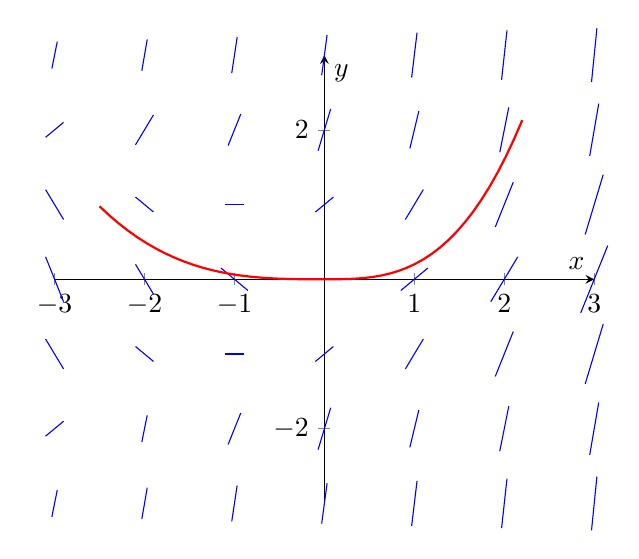
\begin{tikzpicture}
    \begin{axis}[xmin = -3, xmax = 3, ymin = -3, ymax = 3, axis lines = 
    center, xlabel = $x$, ylabel = $y$, clip = false]
    \addplot[blue, thin, domain = -3.03:-2.97]{6*(x - -3) + -3};
    \addplot[blue, thin, domain = -3.1:-2.9]{1*(x - -3) + -2};
    \addplot[blue, thin, domain = -3.1:-2.9]{-2*(x - -3) + -1};
    \addplot[blue, thin, domain = -3.1:-2.9]{-3*(x - -3) + 0};
    \addplot[blue, thin, domain = -3.1:-2.9]{-2*(x - -3) + 1};
    \addplot[blue, thin, domain = -3.1:-2.9]{1*(x - -3) + 2};
    \addplot[blue, thin, domain = -3.03:-2.97]{6*(x - -3) + 3};
    \addplot[blue, thin, domain = -2.03:-1.97]{7*(x - -2) + -3};
    \addplot[blue, thin, domain = -2.03:-1.97]{6*(x - -2) + -2};
    \addplot[blue, thin, domain = -2.1:-1.9]{-1*(x - -2) + -1};
    \addplot[blue, thin, domain = -2.1:-1.9]{-2*(x - -2) + 0};
    \addplot[blue, thin, domain = -2.1:-1.9]{-1*(x - -2) + 1};
    \addplot[blue, thin, domain = -2.1:-1.9]{2*(x - -2) + 2};
    \addplot[blue, thin, domain = -2.03:-1.97]{7*(x - -2) + 3};
    \addplot[blue, thin, domain = -1.03:-0.97]{8*(x - -1) + -3};
    \addplot[blue, thin, domain = -1.07:-0.93]{3*(x - -1) + -2};
    \addplot[blue, thin, domain = -1.1:-0.9]{0*(x - -1) + -1};
    \addplot[blue, thin, domain = -1.15:-0.85]{-1*(x - -1) + 0};
    \addplot[blue, thin, domain = -1.1:-0.9]{0*(x - -1) + 1};
    \addplot[blue, thin, domain = -1.07:-0.93]{3*(x - -1) + 2};
    \addplot[blue, thin, domain = -1.03:-0.97]{8*(x - -1) + 3};
    \addplot[blue, thin, domain = -0.03:0.03]{9*x + -3};
    \addplot[blue, thin, domain = -0.07:0.07]{4*x + -2};
    \addplot[blue, thin, domain = -0.1:0.1]{1*x + -1};
    \addplot[blue, thin, domain = -0.15:0.15]{0*x + 0};
    \addplot[blue, thin, domain = -0.1:0.1]{1*x + 1};
    \addplot[blue, thin, domain = -0.07:0.07]{4*x + 2};
    \addplot[blue, thin, domain = -0.03:0.03]{9*x + 3};
    \addplot[blue, thin, domain = 0.97:1.03]{10*(x - 1) + -3};
    \addplot[blue, thin, domain = 0.95:1.05]{5*(x - 1) + -2};
    \addplot[blue, thin, domain = 0.9:1.1]{2*(x - 1) + -1};
    \addplot[blue, thin, domain = 0.85:1.15]{1*(x - 1) + 0};
    \addplot[blue, thin, domain = 0.9:1.1]{2*(x - 1) + 1};
    \addplot[blue, thin, domain = 0.95:1.05]{5*(x - 1) + 2};
    \addplot[blue, thin, domain = 0.97:1.03]{10*(x - 1) + 3};
    \addplot[blue, thin, domain = 1.97:2.03]{11*(x - 2) + -3};
    \addplot[blue, thin, domain = 1.95:2.05]{6*(x - 2) + -2};
    \addplot[blue, thin, domain = 1.9:2.1]{3*(x-2) + -1};
    \addplot[blue, thin, domain = 1.85:2.15]{2*(x - 2)};
    \addplot[blue, thin, domain = 1.9:2.1]{3*(x-2) + 1};
    \addplot[blue, thin, domain = 1.95:2.05]{6*(x - 2) + 2};
    \addplot[blue, thin, domain = 1.97:2.03]{11*(x - 2) + 3};
    \addplot[blue, thin, domain = 2.97:3.03]{12*(x - 3) + -3};
    \addplot[blue, thin, domain = 2.95:3.05]{7*(x - 3) + -2};
    \addplot[blue, thin, domain = 2.9:3.1]{4*(x - 3) + -1};
    \addplot[blue, thin, domain = 2.85:3.15]{3*(x - 3)};
    \addplot[blue, thin, domain = 2.9:3.1]{4*(x - 3) + 1};
    \addplot[blue, thin, domain = 2.95:3.05]{7*(x - 3) + 2};
    \addplot[blue, thin, domain = 2.97:3.03]{12*(x - 3) + 3};
    \addplot[red, thick, domain = 0:2.2]{0.2*x^3};
    \addplot[red, thick, domain = -2.5:0]{-0.5*(0.5*x)^3};
    \end{axis}
\end{tikzpicture}
\end{Answer}